
%%%%%%%%%%%%%%%%%%%%%%%%%%%%%%%%%%%%%%%%%%%%%%%%%%%%%%%%%%%%%%%%%%%%%%%%%%%%%%%%%%%%%%%%%%
\documentclass[12pt]{article} %a4paper

\usepackage{graphicx} % to include pictures
\usepackage{subfig} % create subfigures within figures
\usepackage{pdflscape} % e.g. to rotate one page of the document
\usepackage{booktabs} % make better looking tabels with different line types and stuff
\usepackage[left=2.5cm,right=3cm,top=3cm,bottom=2.5cm]{geometry}
\usepackage{fancyhdr} % for pages with custom headers and footers
\usepackage[utf8]{inputenc}
\usepackage{float}
\usepackage{datetime}
\usepackage{natbib}
\usepackage{setspace}
\usepackage{booktabs}
\usepackage{multirow}
\usepackage{amsmath}
\usepackage{hyperref}

\setlength{\parindent}{0.0in}
\setlength{\parskip}{1ex plus 0.5ex minus 0.2ex}
\mmddyyyydate
%%%%%%%%%%%%%%%%%%%%%%%%%%%%%%%%%%%%%%%%%%%%%%%%%%%%%%%%%%%%%%%%%%%%%%%%%%%%%%%%%%%%%%%%%%


\begin{document} 

\title{Identifying Equivalent State Bills through Text Reuse. \large Subtitle.}
\date{\today}
\author{}

\maketitle

\begin{abstract}
Much research has been focused on the diffusion of policy ideas in US state
legislatures. Most of this research uses hand coded data sets that identify
equivalent bills and analyze patterns of adoption of these bills. Bills on
equivalent policies often contain the same language, since legislators use past
legislation from other states or model legislation from interest groups as
templates when drafting new bills or model legislation from interest groups. In
this paper we evaluate the effectives of text reuse measures to detect bills
that address the same policy issues. We find that... 
\end{abstract}

\section{Introduction}

Research on public policy adoption and diffusion has conventionally relied on modest hand-coded datasets encode when one or a handful of policies were adopted by each jurisdiction \citep{boehmke2012}. Scholars of public policy diffusion have recently turned their attention to the empirical identification of emulation ties connecting policy jurisdictions \citep{volden2006,boehmke2009,desmarais2015,garrett2015}. Identifying instances of policy emulation and explicit diffusion ties opens policy diffusion scholarship to an entirely new set of questions and theories that can be approached empirically. In this paper we draw upon a massive and nearly all-encompassing source of data from which to infer diffusion ties -- the text of legislation. If the computer-based analysis of bill text can be tuned to successfully identify policy adoption and emulation, we will be able to vastly scale up both the scale of data gathered and the precision of diffusion inferences.


How ever, it is not clear, how well text reuse is suited to to detect real
policy diffusion. There are several complications that we are addressing in this
paper. First, every bill has procedural content that is not related to the
policy content of the bill. Since every state legislature has a set of such
standard or boiler plate text in each bill, there will be significant text reuse
between bills in the same state and possibly also between bills from different
states. Second, it is not obvious how much text reuse will mean substantive

policy overlap. Given that each bill pair has a continuous proportion of
overlapping text, setting the threshold too low might mean to classify bills as
equivalent that are only in the same policy area, or are on a similar issue, but
are opposed in content. On the other hand, setting the threshold too high could
mean overlooking equivalent bills because of small insignificant changes to the
text. 

In this paper we address these issues and evaluate how much policy overlap can
be detected using text reuse measures. Following Wilkerson et al. (2015) we use
supervised machine learning to separate boiler plate from substantive text. We
further more use an original data set on policy diffusion to evaluate how much
equivalent policy can be detected using measures of text reuse. Using the system
developed by Burges et al. (2015) we calculate text reuse scores for all pairs
of bills in our dataset. 

We will then assess the scientific value of the text reuse scores in several different ways. First, we use topic modeling on the discovered reused text sequences to assess the content of the matching text. Second, we investigate the relationship between the ideological distance of the legislators that proposed two bills and the text reuse scores between these bills. Third, we assess the how well policy diffusion networks that have been established by previous research can be discovered using the amount of text reuse between states. And fourth, we use data on equivalent bills collected by the National Council of State Legislatures to build an evaluation data set containing true policy overlap to assess the accuracy of text reuse in predicting policy overlap.

This work has several important implications. First, it allows us to estimate,
how policies are transferred between states. Do state legislators work mainly
from templates from other states or interest groups, or to what extent do
legislators draft their own bill text. Furthermore, text reuse is a relatively
simple metric to calculate for large amounts of text. Previous scholars of
policy diffusion mainly relied on case studies or manually coded data sets of
policy diffusion in few policy areas. If working copying text forms a
significant portion of how legislators adopt policies from other states, text
reuse can be used to easily gather comprehensive data sets on policy diffusion. 


\section{Background}

Public policy diffusion -- the process by which policymakers emulate the policies implemented outside of their jurisdictions -- is a firmly established area of research in both Comparative \citep{simmons2004,gilardi2009} and American politics \citep{walker1969,berry1990,shipan2006,nicholson-crotty2009}. Until recently, policy diffusion studies have deployed quantitative research designs in which the relational component of policy diffusion (i.e., which jurisdiction is being emulated in a given diffusion instance), has been treated as completely unobservable or assumed to align with the geographic adjacency network (i.e., jurisdictions only emulate their geographic neighbors) \citep{volden2006,boehmke2009}. Recognizing the limitations in this approach, scholars have recently taken on the task of directly measuring the latent networks through which policies diffuse. \cite{desmarais2015} apply network inference algorithms to US state adoption sequences in over 100 policy domains to empirically infer the underlying network through which policies diffuse. \cite{garrett2015} analyze the text of US state legislation to measure the diffusion of policy in one domain -- restrictions on insurance coverage for abortion -- and identify the influence of model legislation, as introduced by interest groups.

Previous research on policy diffusion relies almost exclusively on small subsamples of legislation and hand coded data. Little work has been invested in investigating automated ways of detecting equivalent bills in order to measure policy diffusion. 
\citet{wilkerson2015tracing} use the Smith-Waterman local alignment algorithm 
\citep{smith1981identification} to detect overlapping language in congressional bills in order to trace policy ideas through the legislative process of the US congress. 

\subsection{Tasks}
\begin{itemize}
\item Discuss and find some literature on copying legislative language: 
    \begin{itemize}
        \item Interest groups and model legislation
        \item Legislator's resources
    \end{itemize}
\item Policy diffusion (FL expand paragraph)
\item Text re-use in CBP in bills 
\item Text re-use in general
\item Alignment (FL expand review of Wilkerson et al)
\item Discussion of text-based classification
\end{itemize}

\section{Data}

We will rely on two main data sources to assess the reliability of text reuse to
identify substantively equivalent bills. 

\textit{Bill text}\\
In order to calculate the alignment scores between bills, we rely on a database collected by Burgess et al. (2015) and the Sunlight foundation. This data base contains approximately 500,000 bills from 2008 to 2015. The available metadata for the bills includes a timestamp for introduction and approval of the bill, the name and party affiliation of the sponsor(s), the state and the bill id.  This collection of bills is based on all bills that are available through the \url{openstates.org} API. Open states is a website maintained by the Sunlight Foundation, in order to increase transparency in state politics. The Sunlight Foundation use web scrapers to access all bills that are available on the websites of legislatures in all US states. This includes enacted legislation as well as bill that is still in the legislative process, or where not enacted. The database contains the bill text as well as additional information on the legislative process for the bill. We have the first and the last version of the bill text, the sponsor of the bill and all legislative action that was taken on the bill. 

\textit{Alignments}\\
The alignment scores are calculated using the affine version of the local alignment algorithm proposed by \citet{smith1981identification} in order to match genetic sequences. The same algorithm has been used by \citet{wilkerson2015tracing} to trace bills through the legislative process in congress. When considering two bills, the algorithm treats each bill as a sequence of words and tries to find the best alignment between these two sequences. \citet{wilkerson2015tracing} split the bills into sections and search for text reuse across sections. Since this results in about 7 billion possible pairs, first filter out pairs that don't have an exact match of a sequence of at least ten words. We encounter the same problem in our analysis to a greater extent. Assuming each bill consists of ten sections on average, there would be approximately $1.25 * 10^{12}$ possible pairs of sections. 

In order to assess the computational burden the local alignment algorithm poses we test the implementation of the alignment algorithm (Burgess et al. 2015) on a set of 1000 randomly selected bills. In a first pass we calculate the alignments  between all pairs of the full bills (not divided into sections). Figure \ref{fig:time_size} displays the relationship between bill length and computation time. As expected the time increases exponentially with the length of the bills. Figure \ref{fig:time} displays a histogram of the logarithm of the computation time (in seconds). Computation time varies between $0.001s$ and $1,650s$ with $75\%$ of the distribution below $0.1s$ and a median time of $0.03s$.  This shows that an exhaustive comparison of just the full bills (not separated into sections) would take about 100 years on a single machine.

\begin{figure}[ht!]
    \makebox[\textwidth]{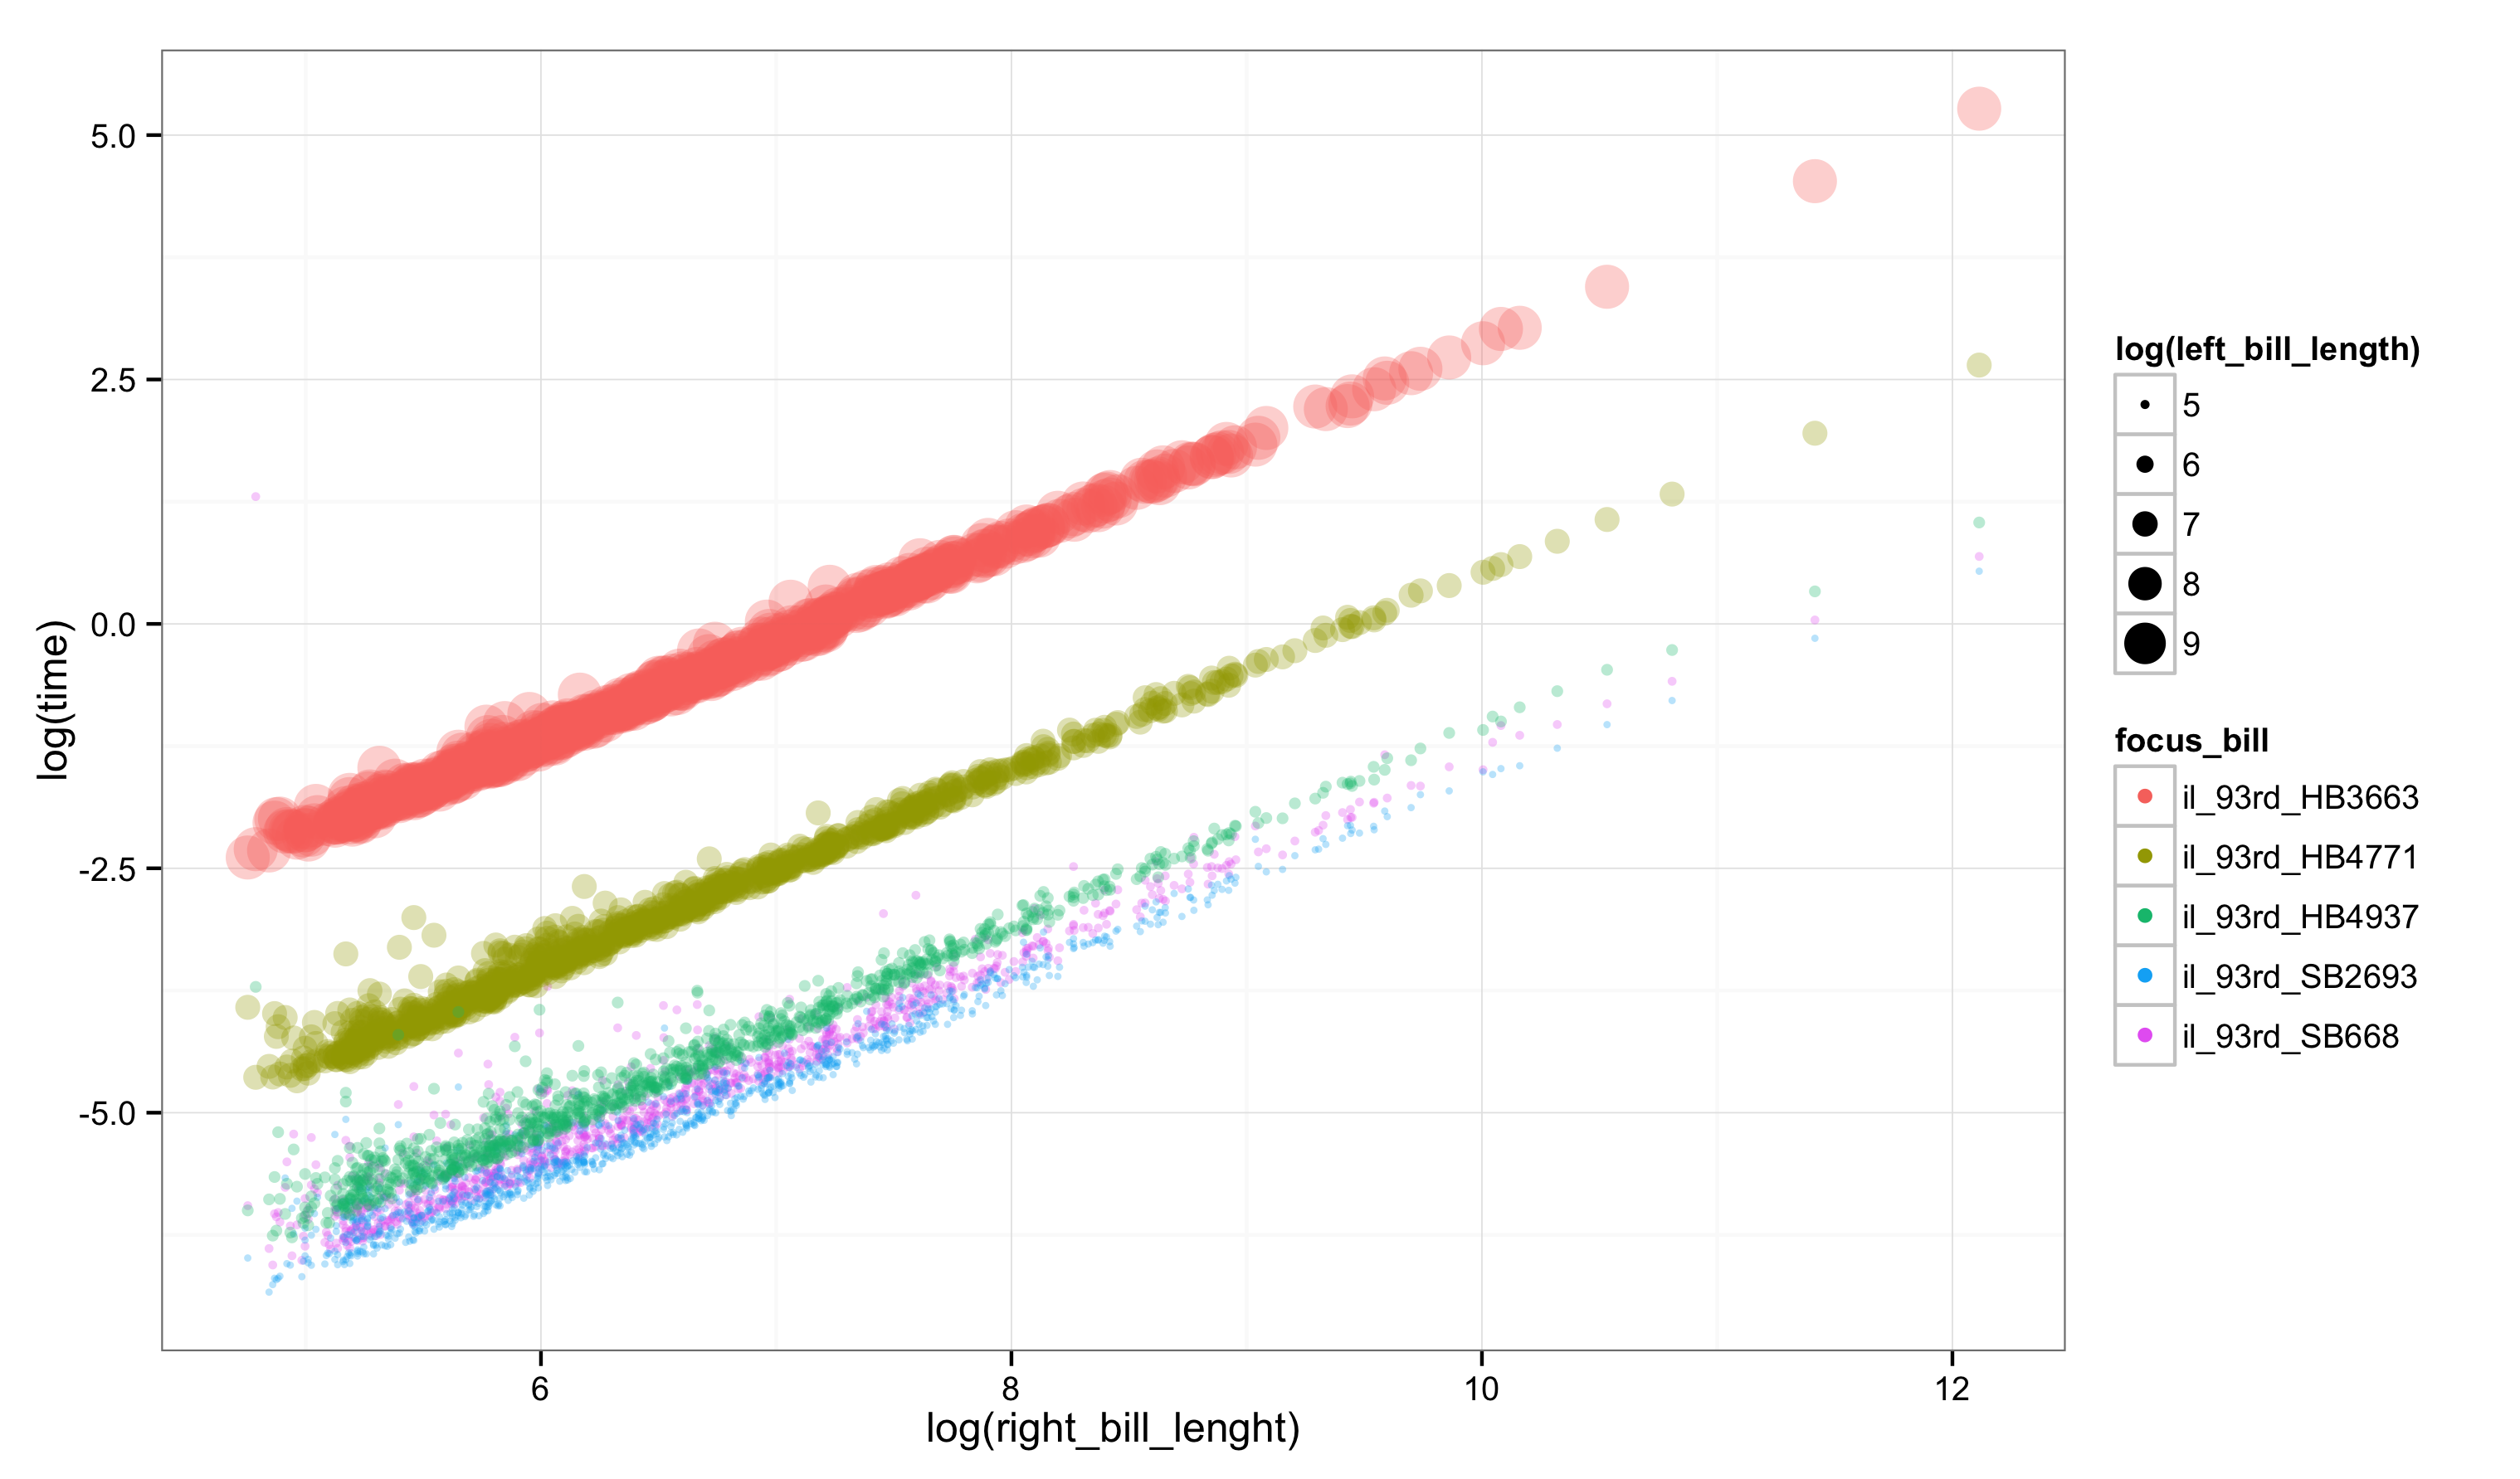
\includegraphics[width=\textwidth]{figures/time_size_selection.png}}
\caption{Computation time for selection of bills. The Colors correspond to five selected bills (focus bill or left bill). For each of the bills, the best alignment with 1000 randomly selected bills (right bills) are calculated. The size of the dots corresponds to the logarithm of the length of the focus bill (in number of words), the x-axis corresponds to the logarithm of the size of the comparison bill and the y-axis corresponds to the logarithm of the computation time (in seconds).}
\label{fig:time_size}
\end{figure}

\begin{figure}[ht!]
    \makebox[\textwidth]{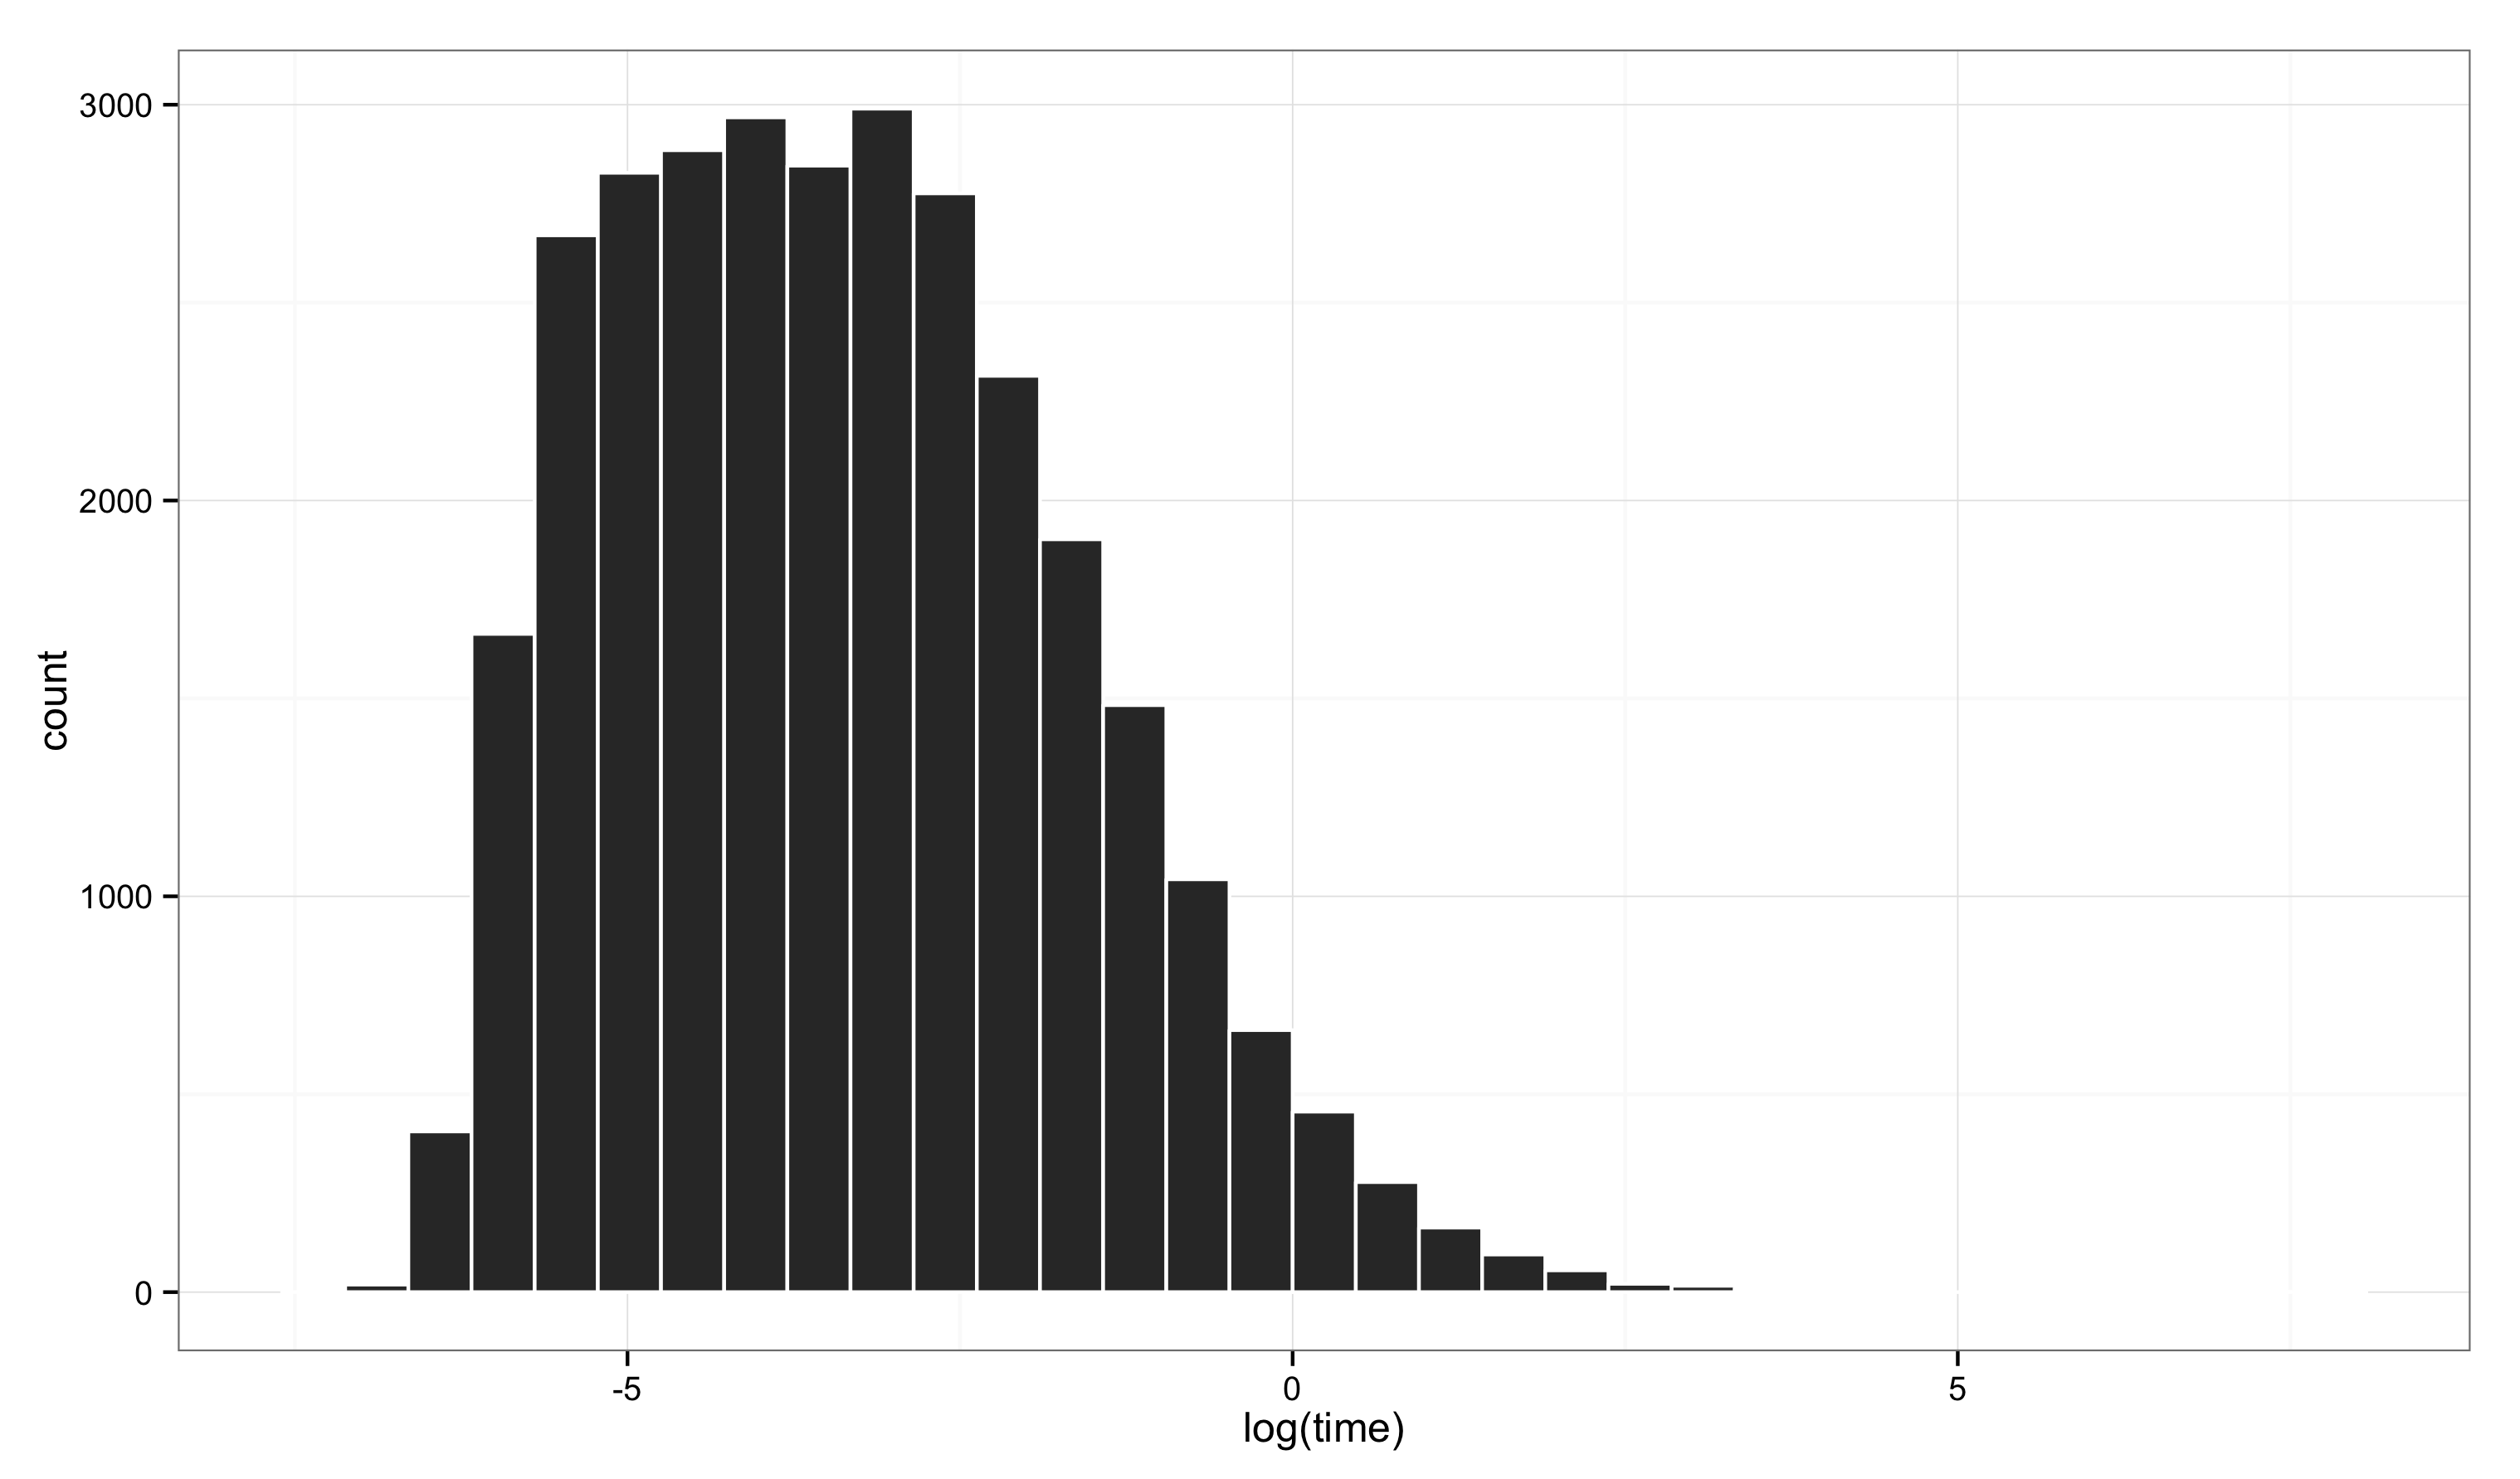
\includegraphics[width=\textwidth]{figures/time.png}}
\caption{Histogram of computation time for all analyzed bills.}
\label{fig:time} 
\end{figure}

Since for this calculation there is no minimum threshold (as in \citet{wilkerson2015tracing} minimum of 5 matching 10-grams). Alignments between almost all bills are found and most of the alignments are procedural language. This is apparent in Figure \ref{fig:state_to_state} which displays the average alignment score for bills from Illinois (left panel) and Washington (right panel) for all other states in the sampled data set (x-axis). Especially for Illinois there is a much higher alignment score for bills from the same state. This shows that a minimum threshold and a classifier for procedural language are necessary.

\begin{figure}[ht!]
    \makebox[\textwidth]{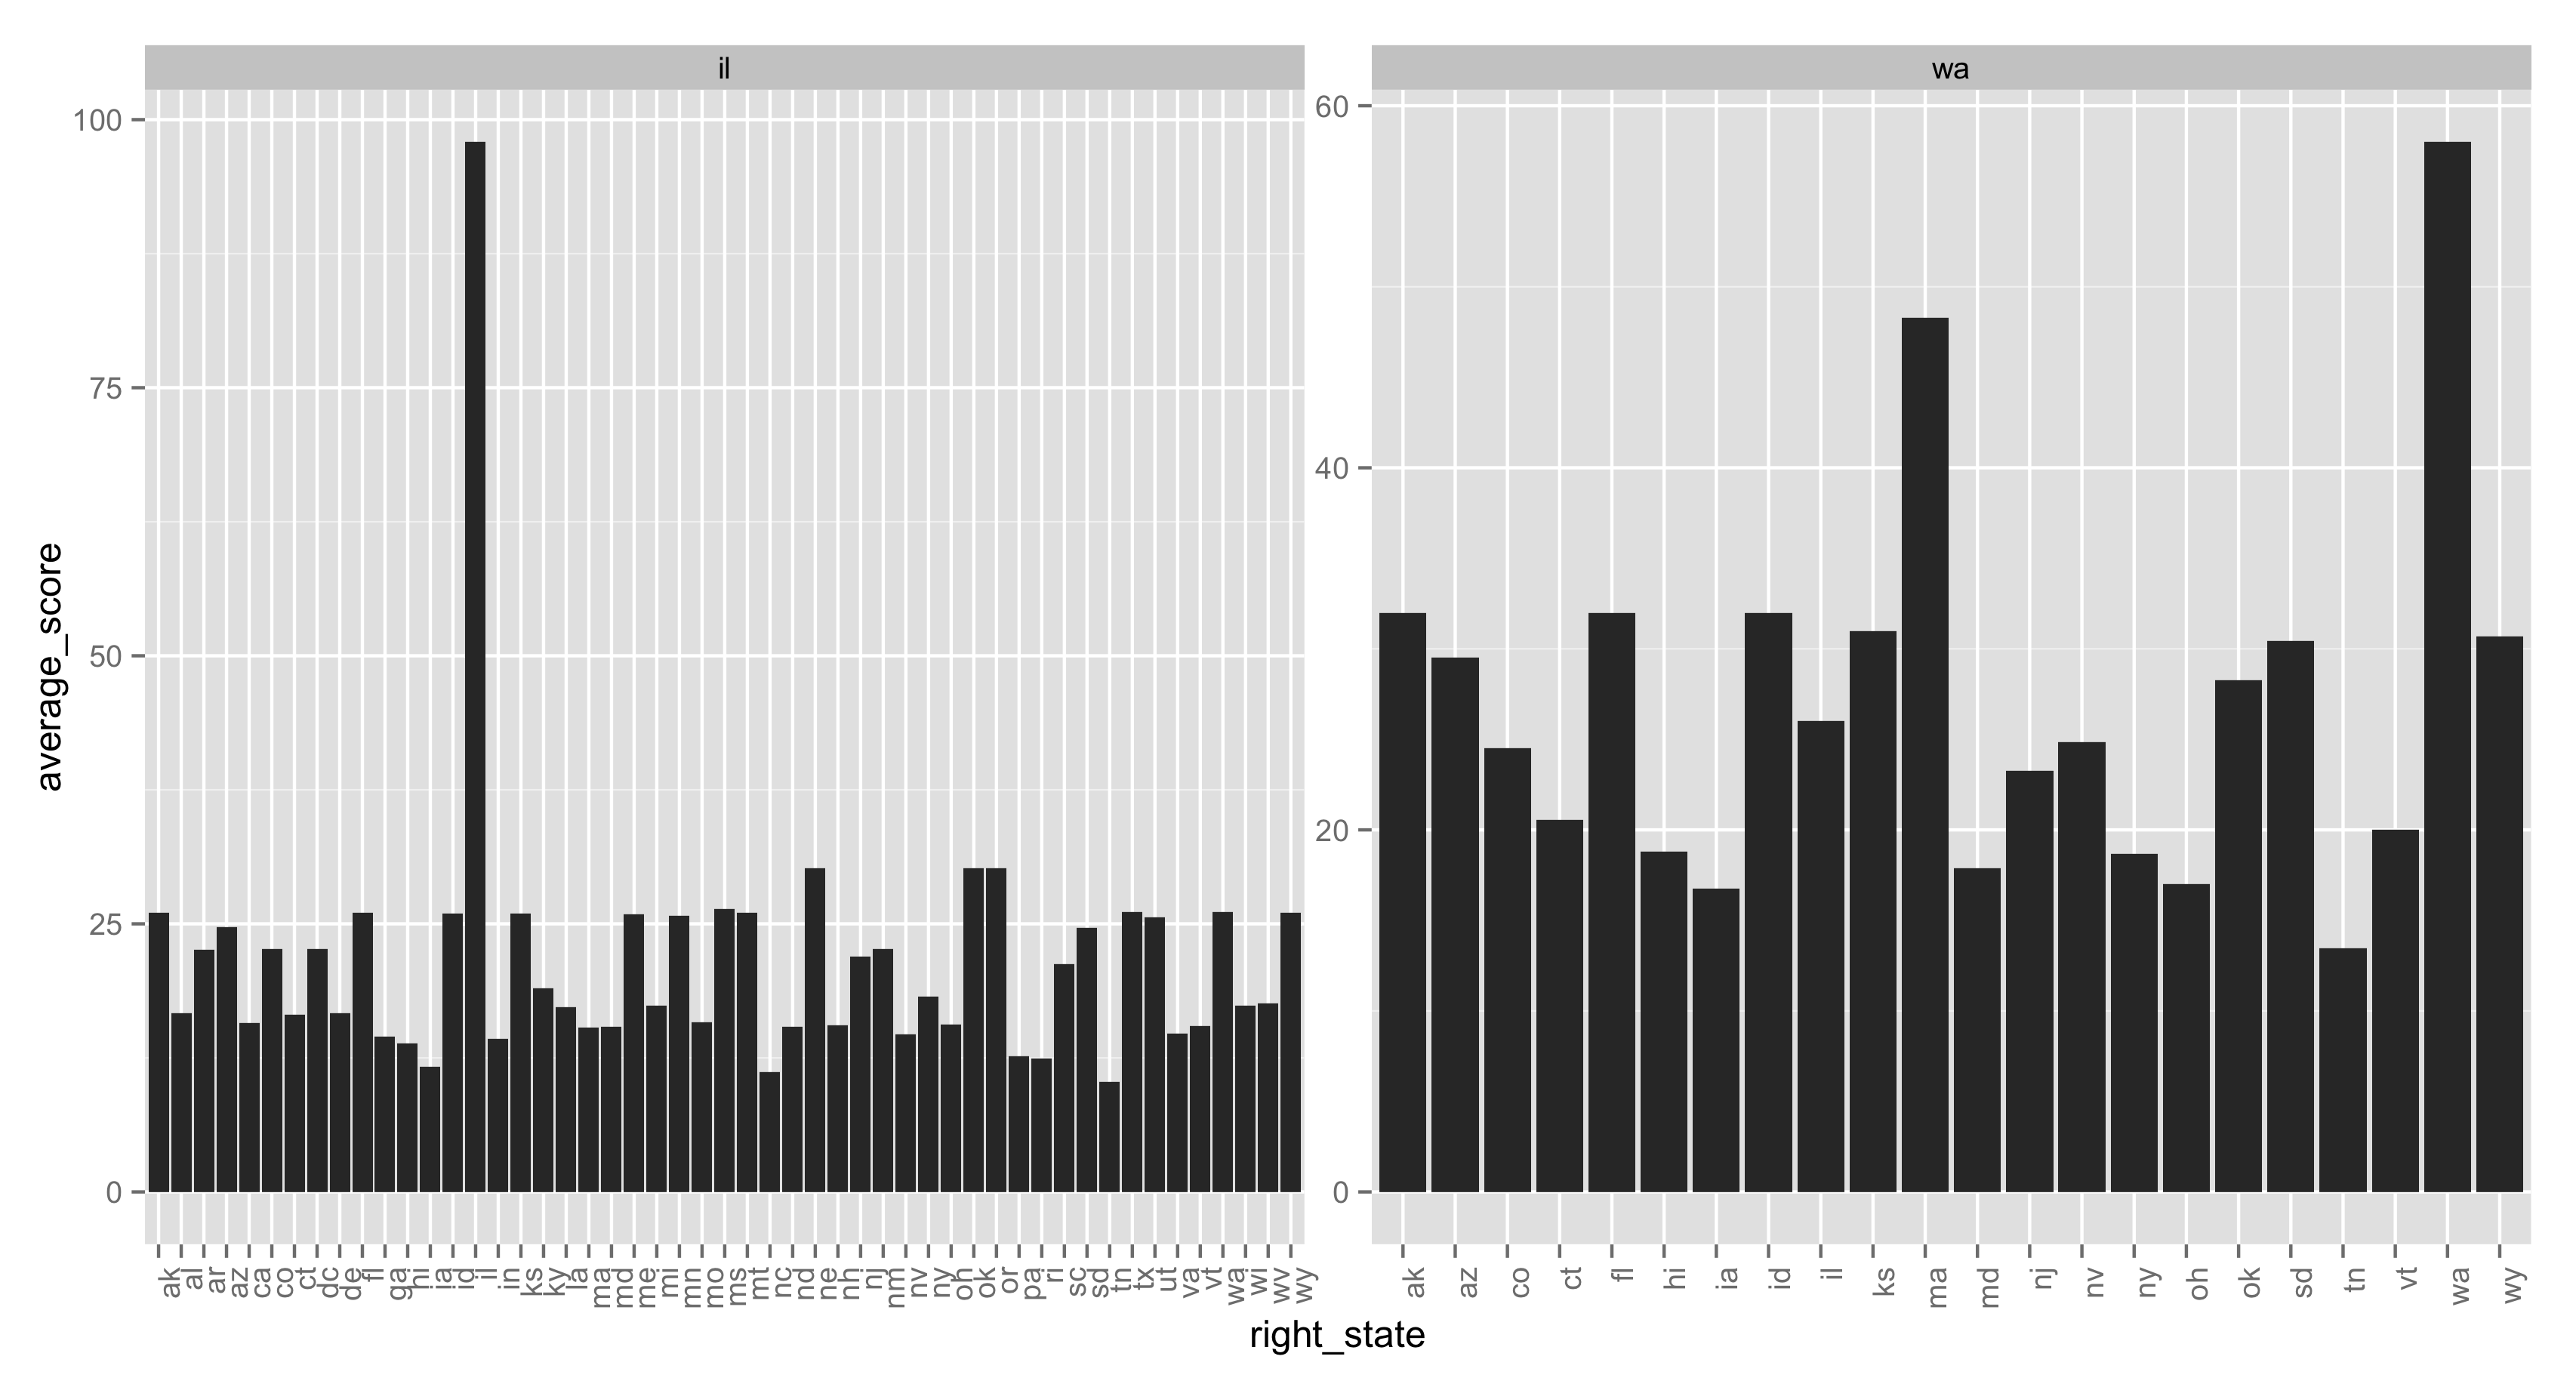
\includegraphics[width=\textwidth]{figures/state_to_state.png}}
\caption{Average alignment scores between states. The left panel corresponds to `left bills' from Illinois, the right panel to bills from Washington. Each bar displays the average score of the best alignment found between bills of the states.}
\label{fig:state_to_state} 
\end{figure}


In order to make the computation more feasible, we rely on a similar strategy as \citet{wilkerson2015tracing}. Our bills are stored in an elastic search database wich provides a variety of search algorithms that are designed to find similar documents. Since seaching the whole database for the full document is very time consuming the following search algorithm is used to first find a pre-selection of similar bills that are then exhaustively checked for text reuse:

\begin{enumerate}
\item All bills are stored in the database in n-grams of size 2-5
\item Select the 25 n-grams with the highest tf-idf score in the query document
\item Calculate a score slightly adapted cosine similarity score between the selected n-gram vector and all full document n-gram vectors in the database\footnote{See \url{https://lucene.apache.org/core/4_9_0/core/org/apache/lucene/search/similarities/TFIDFSimilarity.html} for details on the similarity scoring in Elastic Search}
\end{enumerate}

\subsection*{Tasks}

\begin{itemize}
    \item For the 1000 bill sample, retrieve the 100 most similar bills from the database 
    \item Calculate the alignments between the focus bills and the retrieved bills
    \item Assess the relationship of the search score with the alignment scores
\end{itemize}

\textit{Ideological Scores}\\
For the ideological matching, we rely on latent ideology scores measured by \citep{shor2011}. The data set contains scores for 20738 legislators from 50 state legislatures as well as their party affiliation and their time in office. 

We additionally construct a validation dataset of equivalent bills from information obtained from the National Conference of State Legislatures (NCSL). The NCSL publishes summary tables on specific policies, citing the relevant bills or sections in the state statutes of the states that have implemented regulations on this policy. We collected all these tables, and extracted all bills that address the same policy measure and that overlap with the time frame covered by our bill database.


\subsection{Tasks}
\begin{itemize}
\item Scrape Google urls for NCSL tables (FL) -- lower priority
    \begin{enumerate}
        \item Scraped 64 urls. 
        \item Can't get around the Google API limitation yet. Also get blocked when trying to scrape the search result.
    \end{enumerate}

\item Extract state  \& bill \# from tables (FL) -- lower priority
    \begin{enumerate}
        \item Didn't do this yet, let's first check how many are potentially suitable and then probably better to do by hand
    \end{enumerate}
\item See tasks in analysis -- create metadata file and dyadic file, then put them on the ACI (FL).
    \begin{enumerate}
        \item We have a preliminary dyadic file for all similar bill pairs and their alignment scores (this is from the LID approach: each bill is only compared to the 100 most similar ones)
        \item Matt transfering the database to a new server at the moment, it is therefore unavailable. Should be online again sometime today.
    \end{enumerate}
\item Store MALP data on ACI and make sure the identifiers match those in the bill data (FL). 
    \begin{enumerate}
        \item data is on aci
        \item Legislators can be matched by Name, State, Pary and Term. This information should be contained in the database. If not, the open state api has a legislator search method, that returns all necessary information.
    \end{enumerate}
\item Put policy diffusion data in project folder on ACI (BD).
\end{itemize}

\section{Analysis}
 Below we list X separate analyses designed to test the degree to which measuring text reuse measures policy overlap/diffusion. 

\begin{itemize}
\item We use statistical topic modeling to assess the major content areas represented by the text identified in the alignment algorithm. We consider whether the resultant topics align with policy areas.
\item The Measuring American Legislators Project (MALP) provides data that we will use to assess the significance of text re-use in US state legislation \citet{shor2011}. The most recent release of the MALP data covers 1993-2014. The MALP data provide ideological scores of legislators on an annual basis. We conduct a bill-level statistical network analysis to see whether the rate of bill-to-bill alignment is positively related to the ideological similarity of their sponsors.
\item We conduct a state-level analysis to see whether the volume of state-to-state text alignment is positively related to the policy diffusion networks inferred in \citet{desmarais2015}.
\end{itemize}

\subsection{Diffusion networks and Text re-use}

To evaluate whether text re-use corresponds to the transfer of policy, we test whether the presence of a diffusion network tie between two states is a predictor of text reuse. We use the policy diffusion networks inferred in \citet{desmarais2015}. We use [FL FILL IN] to measure the incidence of dyadic text alignment between all state bills covering the time period 200--[??]. For each bill, we first gather the 100 closest bills based on cosine similarity in the term vectors characterizing the bills. We then represent a dyad of bills by the text alignments between them. For each state-pair we calculate the number of alignments between bills from each state. The median number of alignments between states is 3,491 with a mean of 6,309 and standard deviation of 8,809. The ``Diffusion Ties'' variable measures the number of diffusion edges between states in the 2008 diffusion network, as measured by \citet{desmarais2015}. The number of diffusion edges between two states is either 0, 1, or 2. The diffusion network in 2008 is inferred using policy adoptions in the 35 years preceding (and excluding) 2008. As such, we do not risk double-counting bills in the policy adoption and text re-use data. There is one observation in the analysis for each of the 1,225 unique state-pairs. Since this is dyadic data, we use a matrix permutation method, quadratic assignment procedure, to calculate $p$-values \citep{krackhardt1988}. As a robustness check, we run the model with both the identity and log link.\footnote{The $p$-values were calculated using 5,000 random matrix permutations.}

\begin{table}[ht]
\centering
\begin{tabular}{rrrrr}
\hline
& \multicolumn{2}{c}{Identity Link} & \multicolumn{2}{c}{Log Link} \\
  \hline
 & Coefficient & p-value & Coefficient & p-value \\ 
  \hline
Intercept & 5717.18 & 0.0000 & 8.0431 & 0.0000 \\ 
  Diffusion Ties & 2417.00 & 0.0308 & 0.3288 & 0.0452 \\ 
   \hline
\end{tabular}
\caption{Predicting number of alignments in legislation across states with diffusion ties. Coefficients calculated with OLS regression. $p$-values based on 5,000 QAP permuations.}
\label{tab:qap.diffusion}
\end{table}

Results of the simple dyadic regression are presented in Table \ref{tab:qap.diffusion}. In both specifications there is a positive relationship between the number of diffusion ties and the number of alignments, and the relationship is statistically significant at the 0.05 level (two-tailed). Furthermore, the magnitudes of the relationships are substantively significant. A shift from the minimum to the maximum number of diffusion ties corresponds to more than a half of a standard deviation increase in the expected number of cross-state alignments. On the log scale, the addition of a diffusion tie corresponds to a 40\% increase in the expected number of cross-state alignments.\footnote{Calculated as $100\times \left[ \exp(0.3288)-1\right] = 38.93$}. 



\subsection{Tasks}
\begin{itemize}
\item Develop bill metadata dataset (FL)
\begin{itemize}
\item unique bill identifier
\item sponsor identifier from  MALP data
\item state identifier
\item chamber identifier
\item Introduction date
\item Anything else, even if some is missing (status, committees, etc)
\end{itemize}
\item Develop bill-to-bill edgelists (FL)
\begin{itemize}
\item Sparse dyadic dataset (i.e., no observations when there is 0 alignment/overlap)
\item alignment score(s)
\item name of a text file in which aligned text is stored
\end{itemize}
\item Topic models, possibly of a relational form, applied to aligned text
\item Computationally intensive analysis of bill-to-bill alignment and sponsor ideology.
\begin{itemize}
\item Get big sample of bills
\item Assess relationship between alignment between bills and ideological similarity between sponsors
\end{itemize}
\item Analysis of alignment aggregated at the state level.
\begin{itemize}
\item How do we score overlap at the bill and state level?
\end{itemize}

\end{itemize}


\bibliographystyle{chicago}
\bibliography{bibliography}


\end{document}











